%++++++++++++++++++++++++++++++++++++++++
% Don't modify this section unless you know what you're doing!
\documentclass[letterpaper,12pt]{article}
\usepackage{tabularx} % extra features for tabular environment
\usepackage{amsmath}  % improve math presentation

\usepackage{graphicx}
\graphicspath{{images/}}
\usepackage[section]{placeins}

\usepackage[margin=1in,letterpaper]{geometry} % decreases margins
\usepackage{cite} % takes care of citations
\usepackage[final]{hyperref} % adds hyper links inside the generated pdf file
\hypersetup{
	colorlinks=true,       % false: boxed links; true: colored links
	linkcolor=blue,        % color of internal links
	citecolor=blue,        % color of links to bibliography
	filecolor=magenta,     % color of file links
	urlcolor=blue         
}
%++++++++++++++++++++++++++++++++++++++++
\usepackage[UKenglish]{babel}% http://ctan.org/pkg/babel


\begin{document}

\title{Life in the trenches}
\author{Max Sepulveda}
\date{\today}
\maketitle

\begin{abstract}
The objective of this paper is to present the author's reflections on the question: ``The worst aspect of life in the trenches was boredom''.

\end{abstract}

\section{Main part}

While it is true that boredom was a really important aspect of the life in the trenches, most of the days the soldiers weren't even into battle or doing anything interesting, I don't really agree with this statement.\\

Let me explain why, boredom was a really bad thing but even though you were only some days in the trenches fighting really bad things could happen there (gas attacks,shrapnel from bombs, trench foot, lice, rats). \\

Those, in my opinion, are far worse than boredom, some may kill you painfully and slowly or you could even watch your friends die. 
What about the food? Rats would contaminate it or eat it, the food rations were good but everything could go wrong with some rats, and a lot of people were in constant fear due to this. \\

In conclusion, I don't agree with this statement due to there being many more aspects of life which are worse and more frightening, boredom won’t kill you but gas attacks and shrapnel will.

\nocite{whatwas}
\nocite{photos}

\pagebreak

\section{Daily Life}

\begin{figure}[!htb] 
        % read manual to see what [ht] means and for other possible options
        \centering 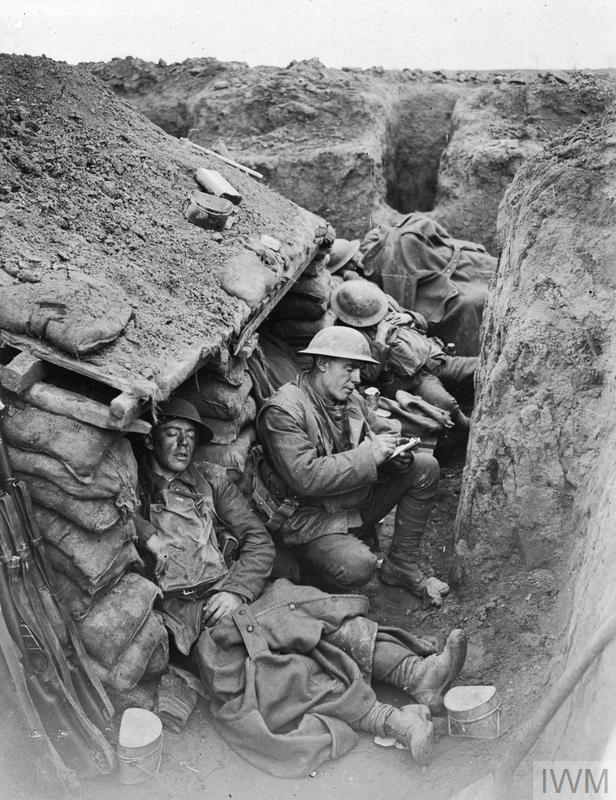
\includegraphics[width=0.5\columnwidth]{large_000000}
        % note that in above figure file name, "sr_setup",
        % the file extension is missing. LaTeX is smart enough to find
        % apropriate one (i.e. pdf, png, etc.)
        % You can add this extention yourself as it seen below
        % both notations are correct but above has more flexibility
        %\includegraphics[width=1.0\columnwidth]{sr_setup.pdf}
        \caption{
                \label{fig:trenche} % spaces are big no-no withing labels
                % things like fig: are optional in the label but it helps
                % to orient yourself when you have multiple figures,
                % equations and tables
                The First World War 1914 - 1918: The Western Front.
        }
\end{figure}



\section{Bibliography}

\begin{thebibliography}{99}

\bibitem{whatwas}
What was life like in a World War One trench?
    \href{https://www.bbc.co.uk/bitesize/topics/zqhyb9q/articles/z8sssbk}{https://www.bbc.co.uk/bitesize/topics/zqhyb9q/articles/z8sssbk}

\bibitem{photos}
10 photos of life in the trenches
    \href{https://www.iwm.org.uk/history/10-photos-of-life-in-the-trenches}{https://www.iwm.org.uk/history/10-photos-of-life-in-the-trenches}


\end{thebibliography}


\end{document}
